\documentclass[twoside]{book}

% Packages required by doxygen
\usepackage{calc}
\usepackage{doxygen}
\usepackage{graphicx}
\usepackage[utf8]{inputenc}
\usepackage{makeidx}
\usepackage{multicol}
\usepackage{multirow}
\usepackage{textcomp}
\usepackage[table]{xcolor}

% Font selection
\usepackage[T1]{fontenc}
\usepackage{mathptmx}
\usepackage[scaled=.90]{helvet}
\usepackage{courier}
\usepackage{amssymb}
\usepackage{sectsty}
\renewcommand{\familydefault}{\sfdefault}
\allsectionsfont{%
  \fontseries{bc}\selectfont%
  \color{darkgray}%
}
\renewcommand{\DoxyLabelFont}{%
  \fontseries{bc}\selectfont%
  \color{darkgray}%
}

% Page & text layout
\usepackage{geometry}
\geometry{%
  a4paper,%
  top=2.5cm,%
  bottom=2.5cm,%
  left=2.5cm,%
  right=2.5cm%
}
\tolerance=750
\hfuzz=15pt
\hbadness=750
\setlength{\emergencystretch}{15pt}
\setlength{\parindent}{0cm}
\setlength{\parskip}{0.2cm}
\makeatletter
\renewcommand{\paragraph}{%
  \@startsection{paragraph}{4}{0ex}{-1.0ex}{1.0ex}{%
    \normalfont\normalsize\bfseries\SS@parafont%
  }%
}
\renewcommand{\subparagraph}{%
  \@startsection{subparagraph}{5}{0ex}{-1.0ex}{1.0ex}{%
    \normalfont\normalsize\bfseries\SS@subparafont%
  }%
}
\makeatother

% Headers & footers
\usepackage{fancyhdr}
\pagestyle{fancyplain}
\fancyhead[LE]{\fancyplain{}{\bfseries\thepage}}
\fancyhead[CE]{\fancyplain{}{}}
\fancyhead[RE]{\fancyplain{}{\bfseries\leftmark}}
\fancyhead[LO]{\fancyplain{}{\bfseries\rightmark}}
\fancyhead[CO]{\fancyplain{}{}}
\fancyhead[RO]{\fancyplain{}{\bfseries\thepage}}
\fancyfoot[LE]{\fancyplain{}{}}
\fancyfoot[CE]{\fancyplain{}{}}
\fancyfoot[RE]{\fancyplain{}{\bfseries\scriptsize Generated on Mon Oct 30 2017 11\-:16\-:33 for My Project by Doxygen }}
\fancyfoot[LO]{\fancyplain{}{\bfseries\scriptsize Generated on Mon Oct 30 2017 11\-:16\-:33 for My Project by Doxygen }}
\fancyfoot[CO]{\fancyplain{}{}}
\fancyfoot[RO]{\fancyplain{}{}}
\renewcommand{\footrulewidth}{0.4pt}
\renewcommand{\chaptermark}[1]{%
  \markboth{#1}{}%
}
\renewcommand{\sectionmark}[1]{%
  \markright{\thesection\ #1}%
}

% Indices & bibliography
\usepackage{natbib}
\usepackage[titles]{tocloft}
\setcounter{tocdepth}{3}
\setcounter{secnumdepth}{5}
\makeindex

% Hyperlinks (required, but should be loaded last)
\usepackage{ifpdf}
\ifpdf
  \usepackage[pdftex,pagebackref=true]{hyperref}
\else
  \usepackage[ps2pdf,pagebackref=true]{hyperref}
\fi
\hypersetup{%
  colorlinks=true,%
  linkcolor=blue,%
  citecolor=blue,%
  unicode%
}

% Custom commands
\newcommand{\clearemptydoublepage}{%
  \newpage{\pagestyle{empty}\cleardoublepage}%
}


%===== C O N T E N T S =====

\begin{document}

% Titlepage & ToC
\hypersetup{pageanchor=false}
\pagenumbering{roman}
\begin{titlepage}
\vspace*{7cm}
\begin{center}%
{\Large My Project }\\
\vspace*{1cm}
{\large Generated by Doxygen 1.8.6}\\
\vspace*{0.5cm}
{\small Mon Oct 30 2017 11:16:33}\\
\end{center}
\end{titlepage}
\clearemptydoublepage
\tableofcontents
\clearemptydoublepage
\pagenumbering{arabic}
\hypersetup{pageanchor=true}

%--- Begin generated contents ---
\chapter{Hierarchical Index}
\section{Class Hierarchy}
This inheritance list is sorted roughly, but not completely, alphabetically\-:\begin{DoxyCompactList}
\item \contentsline{section}{Network}{\pageref{classNetwork}}{}
\item \contentsline{section}{Neuron}{\pageref{classNeuron}}{}
\begin{DoxyCompactList}
\item \contentsline{section}{Excitatory\-Neuron}{\pageref{classExcitatoryNeuron}}{}
\item \contentsline{section}{Inhibitory\-Neuron}{\pageref{classInhibitoryNeuron}}{}
\end{DoxyCompactList}
\end{DoxyCompactList}

\chapter{Class Index}
\section{Class List}
Here are the classes, structs, unions and interfaces with brief descriptions\-:\begin{DoxyCompactList}
\item\contentsline{section}{\hyperlink{classExcitatoryNeuron}{Excitatory\-Neuron} \\*A subclass of \hyperlink{classNeuron}{Neuron} }{\pageref{classExcitatoryNeuron}}{}
\item\contentsline{section}{\hyperlink{classInhibitoryNeuron}{Inhibitory\-Neuron} \\*A subclass of \hyperlink{classNeuron}{Neuron} }{\pageref{classInhibitoryNeuron}}{}
\item\contentsline{section}{\hyperlink{classNetwork}{Network} }{\pageref{classNetwork}}{}
\item\contentsline{section}{\hyperlink{classNeuron}{Neuron} }{\pageref{classNeuron}}{}
\item\contentsline{section}{\hyperlink{classSimulation}{Simulation} }{\pageref{classSimulation}}{}
\end{DoxyCompactList}

\chapter{Class Documentation}
\hypertarget{classExcitatoryNeuron}{\section{Excitatory\-Neuron Class Reference}
\label{classExcitatoryNeuron}\index{Excitatory\-Neuron@{Excitatory\-Neuron}}
}
Inheritance diagram for Excitatory\-Neuron\-:\begin{figure}[H]
\begin{center}
\leavevmode
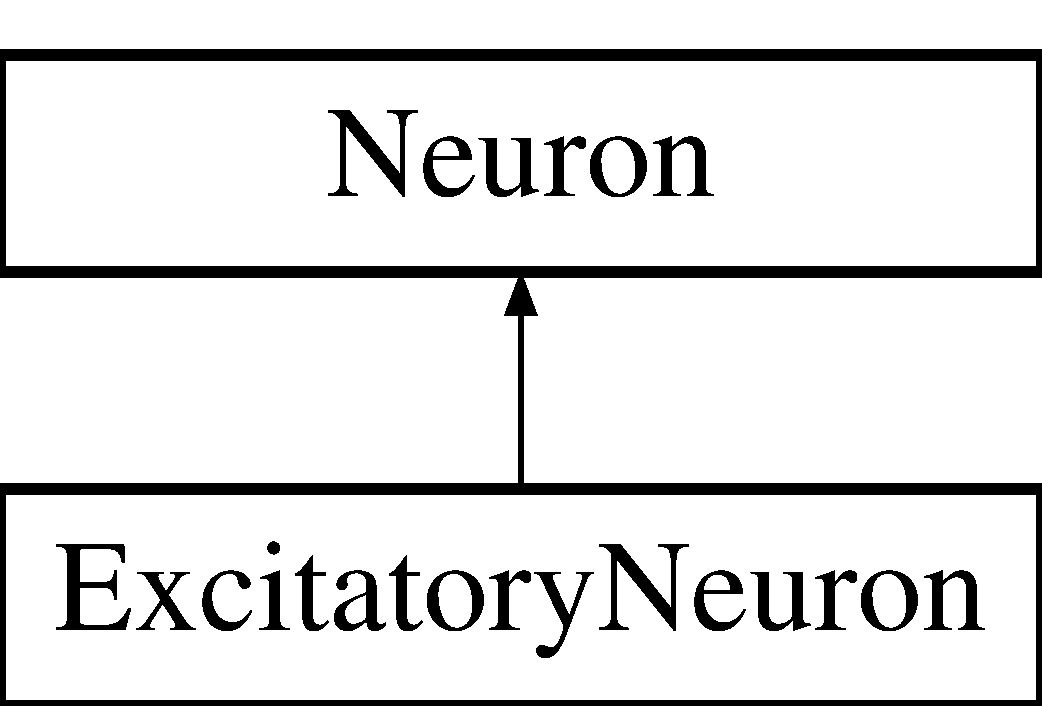
\includegraphics[height=2.000000cm]{classExcitatoryNeuron}
\end{center}
\end{figure}
\subsection*{Public Member Functions}
\begin{DoxyCompactItemize}
\item 
double \hyperlink{classExcitatoryNeuron_a7d38213943753c84022c52db84601e67}{get\-Spike\-Amplitude} () const 
\end{DoxyCompactItemize}


\subsection{Member Function Documentation}
\hypertarget{classExcitatoryNeuron_a7d38213943753c84022c52db84601e67}{\index{Excitatory\-Neuron@{Excitatory\-Neuron}!get\-Spike\-Amplitude@{get\-Spike\-Amplitude}}
\index{get\-Spike\-Amplitude@{get\-Spike\-Amplitude}!ExcitatoryNeuron@{Excitatory\-Neuron}}
\subsubsection[{get\-Spike\-Amplitude}]{\setlength{\rightskip}{0pt plus 5cm}double Excitatory\-Neuron\-::get\-Spike\-Amplitude (
\begin{DoxyParamCaption}
{}
\end{DoxyParamCaption}
) const\hspace{0.3cm}{\ttfamily [virtual]}}}\label{classExcitatoryNeuron_a7d38213943753c84022c52db84601e67}
A virtual method which reads the constant spike amplitude, that differs between inhibitory and excitatory neurons, from the parameter file. (The method is defined for unspecified neurons as well so that the tests of previous versions of the program are still functional, otherwise it could be virtual pure.). \begin{DoxySeeAlso}{See Also}
\hyperlink{classNeuron_a41a81d8527734e59bae39f73fece887f}{update\-Membrane\-Potential()} 
\end{DoxySeeAlso}
\begin{DoxyReturn}{Returns}
the spike amplitudes of the presynaptic neuron, a double 
\end{DoxyReturn}


Reimplemented from \hyperlink{classNeuron_aec2283fbfaba764cd088e6d16b0a74bb}{Neuron}.



The documentation for this class was generated from the following files\-:\begin{DoxyCompactItemize}
\item 
excitatory\-Neuron.\-hpp\item 
excitatory\-Neuron.\-cpp\end{DoxyCompactItemize}

\hypertarget{classInhibitoryNeuron}{\section{Inhibitory\-Neuron Class Reference}
\label{classInhibitoryNeuron}\index{Inhibitory\-Neuron@{Inhibitory\-Neuron}}
}
Inheritance diagram for Inhibitory\-Neuron\-:\begin{figure}[H]
\begin{center}
\leavevmode
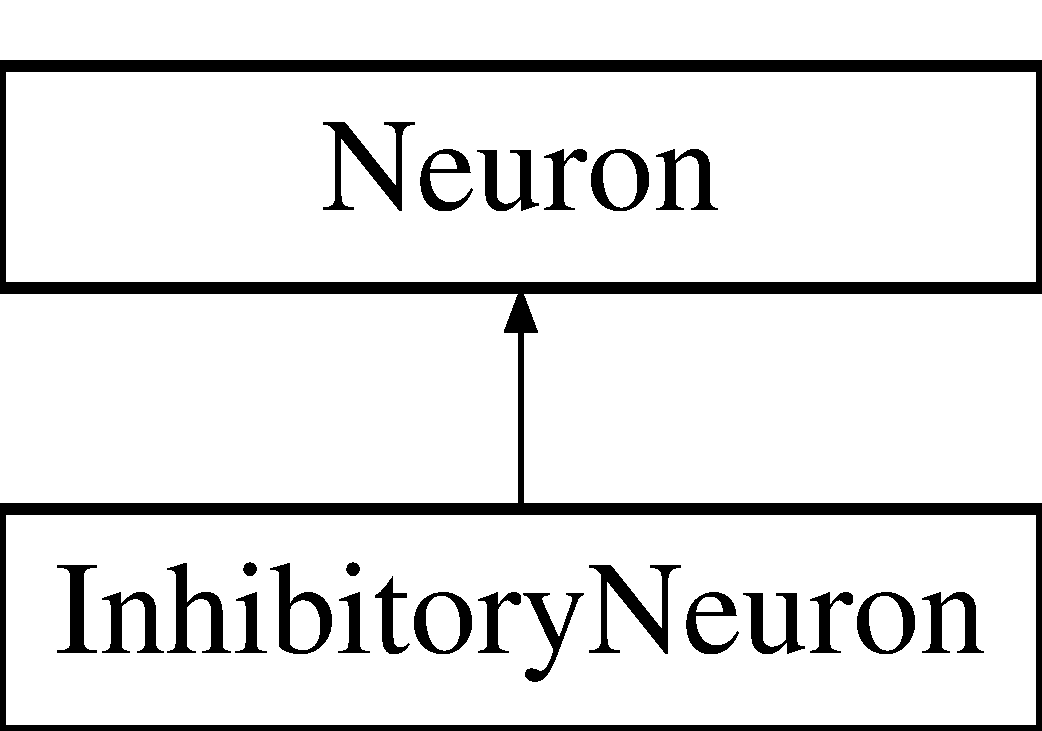
\includegraphics[height=2.000000cm]{classInhibitoryNeuron}
\end{center}
\end{figure}
\subsection*{Public Member Functions}
\begin{DoxyCompactItemize}
\item 
double \hyperlink{classInhibitoryNeuron_a762e2b7bcf64962f764031d991911b7a}{get\-Spike\-Amplitude} () const override
\end{DoxyCompactItemize}


\subsection{Member Function Documentation}
\hypertarget{classInhibitoryNeuron_a762e2b7bcf64962f764031d991911b7a}{\index{Inhibitory\-Neuron@{Inhibitory\-Neuron}!get\-Spike\-Amplitude@{get\-Spike\-Amplitude}}
\index{get\-Spike\-Amplitude@{get\-Spike\-Amplitude}!InhibitoryNeuron@{Inhibitory\-Neuron}}
\subsubsection[{get\-Spike\-Amplitude}]{\setlength{\rightskip}{0pt plus 5cm}double Inhibitory\-Neuron\-::get\-Spike\-Amplitude (
\begin{DoxyParamCaption}
{}
\end{DoxyParamCaption}
) const\hspace{0.3cm}{\ttfamily [override]}, {\ttfamily [virtual]}}}\label{classInhibitoryNeuron_a762e2b7bcf64962f764031d991911b7a}
A virtual method which reads the constant spike amplitude, that differs between inhibitory and excitatory neurons, from the parameter file. (The method is defined for unspecified neurons as well so that the tests of previous versions of the program are still functional, otherwise it could be virtual pure.). \begin{DoxySeeAlso}{See Also}
\hyperlink{classNeuron_a41a81d8527734e59bae39f73fece887f}{update\-Membrane\-Potential()} 
\end{DoxySeeAlso}
\begin{DoxyReturn}{Returns}
the spike amplitudes of the presynaptic neuron, a double 
\end{DoxyReturn}


Reimplemented from \hyperlink{classNeuron_aec2283fbfaba764cd088e6d16b0a74bb}{Neuron}.



The documentation for this class was generated from the following files\-:\begin{DoxyCompactItemize}
\item 
inhibitory\-Neuron.\-hpp\item 
inhibitory\-Neuron.\-cpp\end{DoxyCompactItemize}

\hypertarget{classNetwork}{\section{Network Class Reference}
\label{classNetwork}\index{Network@{Network}}
}
\subsection*{Public Member Functions}
\begin{DoxyCompactItemize}
\item 
\hyperlink{classNetwork_a3cc2fb4f8fa4d507077e8da85ce5a1c8}{Network} ()
\begin{DoxyCompactList}\small\item\em A constructor. \end{DoxyCompactList}\item 
\hypertarget{classNetwork_a7a4e19cdb4bf0c7ecf82baa643831492}{\hyperlink{classNetwork_a7a4e19cdb4bf0c7ecf82baa643831492}{$\sim$\-Network} ()}\label{classNetwork_a7a4e19cdb4bf0c7ecf82baa643831492}

\begin{DoxyCompactList}\small\item\em A destructor which deletes all neurons of the network. \end{DoxyCompactList}\item 
\hypertarget{classNetwork_ab07bb6f6d9020b9eb230551083ea929f}{void \hyperlink{classNetwork_ab07bb6f6d9020b9eb230551083ea929f}{update} ()}\label{classNetwork_ab07bb6f6d9020b9eb230551083ea929f}

\begin{DoxyCompactList}\small\item\em A method updating all of the network's neuron by one step which is used in the main loop. \end{DoxyCompactList}\item 
\hypertarget{classNetwork_a618d267c0962f59027c0d063aa2b4533}{std\-::vector$<$ std\-::vector\\*
$<$ unsigned int $>$ $>$ \hyperlink{classNetwork_a618d267c0962f59027c0d063aa2b4533}{get\-Spike\-Times} ()}\label{classNetwork_a618d267c0962f59027c0d063aa2b4533}

\begin{DoxyCompactList}\small\item\em A getter of the spiking times of all neurons, allows to retreive data. \end{DoxyCompactList}\item 
void \hyperlink{classNetwork_a222e084554183af355833cda07a83877}{print\-Simulation\-Data} (const std\-::string \&name\-Of\-File) const 
\item 
void \hyperlink{classNetwork_a8909c07d0e6e292f5ca54e56a797ebe0}{print\-Simulation\-Data\-Within\-Time\-Interval} (const std\-::string \&name\-Of\-File) const 
\item 
double \hyperlink{classNetwork_ac82435bb56bf5eabfdd3e3f4afadea2b}{get\-Mean\-Spike\-Rate\-In\-Interval} (unsigned int begin\-Interval, unsigned int end\-Interval) const 
\end{DoxyCompactItemize}
\subsection*{Private Member Functions}
\begin{DoxyCompactItemize}
\item 
void \hyperlink{classNetwork_ad28d5206f20213eba2143222c566fb00}{print\-Simulation\-Data} (const std\-::string \&name\-Of\-File, std\-::vector$<$ unsigned int $>$\-::const\-\_\-iterator(Network\-::$\ast$get\-Iterator\-Begin)(unsigned int) const , std\-::vector$<$ unsigned int $>$\-::const\-\_\-iterator(Network\-::$\ast$get\-Iterator\-End)(unsigned int) const ) const 
\item 
std\-::vector$<$ unsigned int $>$\\*
\-::const\-\_\-iterator \hyperlink{classNetwork_a0423144b1411e885884410adb9ff10d4}{get\-Iterator\-To\-Begin} (unsigned int i) const 
\item 
std\-::vector$<$ unsigned int $>$\\*
\-::const\-\_\-iterator \hyperlink{classNetwork_a0289c82fc429d301c1f7b33881b6737d}{get\-Iterator\-To\-End} (unsigned int i) const 
\item 
std\-::vector$<$ unsigned int $>$\\*
\-::const\-\_\-iterator \hyperlink{classNetwork_af437eddac886ac6fced8078885a2cc0a}{get\-Iterator\-To\-Begin\-Interval} (unsigned int i) const 
\item 
\hypertarget{classNetwork_a009cca76442a5f847fd1e227b0427313}{std\-::vector$<$ unsigned int $>$\\*
\-::const\-\_\-iterator {\bfseries get\-Iterator\-To\-End\-Interval} (unsigned int i) const }\label{classNetwork_a009cca76442a5f847fd1e227b0427313}

\end{DoxyCompactItemize}
\subsection*{Private Attributes}
\begin{DoxyCompactItemize}
\item 
\hypertarget{classNetwork_a11dac461892218c2653fccdb761a99aa}{std\-::array$<$ \hyperlink{classNeuron}{Neuron} \\*
$\ast$, T\-O\-T\-A\-L\-\_\-\-N\-U\-M\-B\-E\-R\-\_\-\-O\-F\-\_\-\-N\-E\-U\-R\-O\-N\-S\-\_\-\-N $>$ \hyperlink{classNetwork_a11dac461892218c2653fccdb761a99aa}{neurons}}\label{classNetwork_a11dac461892218c2653fccdb761a99aa}

\begin{DoxyCompactList}\small\item\em A container carrying the neurons forming the network, an array of pointers to neurons. \end{DoxyCompactList}\end{DoxyCompactItemize}


\subsection{Constructor \& Destructor Documentation}
\hypertarget{classNetwork_a3cc2fb4f8fa4d507077e8da85ce5a1c8}{\index{Network@{Network}!Network@{Network}}
\index{Network@{Network}!Network@{Network}}
\subsubsection[{Network}]{\setlength{\rightskip}{0pt plus 5cm}Network\-::\-Network (
\begin{DoxyParamCaption}
{}
\end{DoxyParamCaption}
)}}\label{classNetwork_a3cc2fb4f8fa4d507077e8da85ce5a1c8}


A constructor. 

Initializes a neuron network by creating 12'500 neurons among those 2'500 are inhibitory and the other 10'000 exitatory. Each one of them receives a fixed number of connections from both inhibitory and excitatory presynaptic neuron that are chosen randomly. 

\subsection{Member Function Documentation}
\hypertarget{classNetwork_a0423144b1411e885884410adb9ff10d4}{\index{Network@{Network}!get\-Iterator\-To\-Begin@{get\-Iterator\-To\-Begin}}
\index{get\-Iterator\-To\-Begin@{get\-Iterator\-To\-Begin}!Network@{Network}}
\subsubsection[{get\-Iterator\-To\-Begin}]{\setlength{\rightskip}{0pt plus 5cm}vector$<$ unsigned int $>$\-::const\-\_\-iterator Network\-::get\-Iterator\-To\-Begin (
\begin{DoxyParamCaption}
\item[{unsigned int}]{i}
\end{DoxyParamCaption}
) const\hspace{0.3cm}{\ttfamily [private]}}}\label{classNetwork_a0423144b1411e885884410adb9ff10d4}
An auxiliary function for printing the network's spike times to a file that returns an iterator pointing on neuron i's first spike time. \begin{DoxySeeAlso}{See Also}
print\-Simulation\-Data(const std\-::string\& name\-Of\-File) 
\end{DoxySeeAlso}

\begin{DoxyParams}{Parameters}
{\em neuron} & identifier, an unsigned int \\
\hline
\end{DoxyParams}
\hypertarget{classNetwork_af437eddac886ac6fced8078885a2cc0a}{\index{Network@{Network}!get\-Iterator\-To\-Begin\-Interval@{get\-Iterator\-To\-Begin\-Interval}}
\index{get\-Iterator\-To\-Begin\-Interval@{get\-Iterator\-To\-Begin\-Interval}!Network@{Network}}
\subsubsection[{get\-Iterator\-To\-Begin\-Interval}]{\setlength{\rightskip}{0pt plus 5cm}vector$<$ unsigned int $>$\-::const\-\_\-iterator Network\-::get\-Iterator\-To\-Begin\-Interval (
\begin{DoxyParamCaption}
\item[{unsigned int}]{i}
\end{DoxyParamCaption}
) const\hspace{0.3cm}{\ttfamily [private]}}}\label{classNetwork_af437eddac886ac6fced8078885a2cc0a}
An auxiliary function for printing the network's spike times to a file that returns an iterator pointing on neuron i's first spike time that lies within an interval defined in the parameter file. \begin{DoxySeeAlso}{See Also}
print\-Simulation\-Data(const std\-::string\& name\-Of\-File) 
\end{DoxySeeAlso}

\begin{DoxyParams}{Parameters}
{\em neuron} & identifier, an unsigned int \\
\hline
\end{DoxyParams}
\hypertarget{classNetwork_a0289c82fc429d301c1f7b33881b6737d}{\index{Network@{Network}!get\-Iterator\-To\-End@{get\-Iterator\-To\-End}}
\index{get\-Iterator\-To\-End@{get\-Iterator\-To\-End}!Network@{Network}}
\subsubsection[{get\-Iterator\-To\-End}]{\setlength{\rightskip}{0pt plus 5cm}vector$<$ unsigned int $>$\-::const\-\_\-iterator Network\-::get\-Iterator\-To\-End (
\begin{DoxyParamCaption}
\item[{unsigned int}]{i}
\end{DoxyParamCaption}
) const\hspace{0.3cm}{\ttfamily [private]}}}\label{classNetwork_a0289c82fc429d301c1f7b33881b6737d}
An auxiliary function for printing the network's spike times to a file that returns an iterator pointing on neuron i's last spike time. \begin{DoxySeeAlso}{See Also}
print\-Simulation\-Data(const std\-::string\& name\-Of\-File) 
\end{DoxySeeAlso}

\begin{DoxyParams}{Parameters}
{\em neuron} & identifier, an unsigned int \\
\hline
\end{DoxyParams}
\hypertarget{classNetwork_ac82435bb56bf5eabfdd3e3f4afadea2b}{\index{Network@{Network}!get\-Mean\-Spike\-Rate\-In\-Interval@{get\-Mean\-Spike\-Rate\-In\-Interval}}
\index{get\-Mean\-Spike\-Rate\-In\-Interval@{get\-Mean\-Spike\-Rate\-In\-Interval}!Network@{Network}}
\subsubsection[{get\-Mean\-Spike\-Rate\-In\-Interval}]{\setlength{\rightskip}{0pt plus 5cm}double Network\-::get\-Mean\-Spike\-Rate\-In\-Interval (
\begin{DoxyParamCaption}
\item[{unsigned int}]{begin\-Interval, }
\item[{unsigned int}]{end\-Interval}
\end{DoxyParamCaption}
) const}}\label{classNetwork_ac82435bb56bf5eabfdd3e3f4afadea2b}
Calculates the mean spike rate of the network's neurons in an interval to indicate. 
\begin{DoxyParams}{Parameters}
{\em begin} & of the interval to investigate in steps, an unsigned int \\
\hline
{\em begin} & of the interval to investigate in steps, an unsigned int \\
\hline
\end{DoxyParams}
\hypertarget{classNetwork_a222e084554183af355833cda07a83877}{\index{Network@{Network}!print\-Simulation\-Data@{print\-Simulation\-Data}}
\index{print\-Simulation\-Data@{print\-Simulation\-Data}!Network@{Network}}
\subsubsection[{print\-Simulation\-Data}]{\setlength{\rightskip}{0pt plus 5cm}void Network\-::print\-Simulation\-Data (
\begin{DoxyParamCaption}
\item[{const std\-::string \&}]{name\-Of\-File}
\end{DoxyParamCaption}
) const}}\label{classNetwork_a222e084554183af355833cda07a83877}
Prints each neuron's spike times and neuron id in a file of given name using the private function print simulation data. 
\begin{DoxyParams}{Parameters}
{\em name\-Of\-File,a} & string \\
\hline
\end{DoxyParams}
\hypertarget{classNetwork_ad28d5206f20213eba2143222c566fb00}{\index{Network@{Network}!print\-Simulation\-Data@{print\-Simulation\-Data}}
\index{print\-Simulation\-Data@{print\-Simulation\-Data}!Network@{Network}}
\subsubsection[{print\-Simulation\-Data}]{\setlength{\rightskip}{0pt plus 5cm}void Network\-::print\-Simulation\-Data (
\begin{DoxyParamCaption}
\item[{const std\-::string \&}]{name\-Of\-File, }
\item[{std\-::vector$<$ unsigned int $>$\-::const\-\_\-iterator(Network\-::$\ast$)(unsigned int) const}]{get\-Iterator\-Begin, }
\item[{std\-::vector$<$ unsigned int $>$\-::const\-\_\-iterator(Network\-::$\ast$)(unsigned int) const}]{get\-Iterator\-End}
\end{DoxyParamCaption}
) const\hspace{0.3cm}{\ttfamily [private]}}}\label{classNetwork_ad28d5206f20213eba2143222c566fb00}
An auxiliary function for printing the network's spike times to a file that allows to avoid the duplication of code. \begin{DoxySeeAlso}{See Also}
print\-Simulation\-Data(const std\-::string\& name\-Of\-File) 

\hyperlink{classNetwork_a8909c07d0e6e292f5ca54e56a797ebe0}{print\-Simulation\-Data\-Within\-Time\-Interval} 
\end{DoxySeeAlso}

\begin{DoxyParams}{Parameters}
{\em name\-Of\-File,a} & string \\
\hline
{\em a} & member function that yields an iterator on a vector$<$unsigned int$>$ pointing the first element that is printed \\
\hline
{\em a} & member function that yields an iterator on a vector$<$unsigned int$>$ pointing the last element that is printed \\
\hline
\end{DoxyParams}
\hypertarget{classNetwork_a8909c07d0e6e292f5ca54e56a797ebe0}{\index{Network@{Network}!print\-Simulation\-Data\-Within\-Time\-Interval@{print\-Simulation\-Data\-Within\-Time\-Interval}}
\index{print\-Simulation\-Data\-Within\-Time\-Interval@{print\-Simulation\-Data\-Within\-Time\-Interval}!Network@{Network}}
\subsubsection[{print\-Simulation\-Data\-Within\-Time\-Interval}]{\setlength{\rightskip}{0pt plus 5cm}void Network\-::print\-Simulation\-Data\-Within\-Time\-Interval (
\begin{DoxyParamCaption}
\item[{const std\-::string \&}]{name\-Of\-File}
\end{DoxyParamCaption}
) const}}\label{classNetwork_a8909c07d0e6e292f5ca54e56a797ebe0}
Prints each neuron's spike times that are in an interval defined in the simulation's parameter file and neuron id in a file of given name using the private function print simulation data. 
\begin{DoxyParams}{Parameters}
{\em name\-Of\-File,a} & string \\
\hline
\end{DoxyParams}


The documentation for this class was generated from the following files\-:\begin{DoxyCompactItemize}
\item 
network.\-hpp\item 
network.\-cpp\end{DoxyCompactItemize}

\hypertarget{classNeuron}{\section{Neuron Class Reference}
\label{classNeuron}\index{Neuron@{Neuron}}
}
Inheritance diagram for Neuron\-:\begin{figure}[H]
\begin{center}
\leavevmode
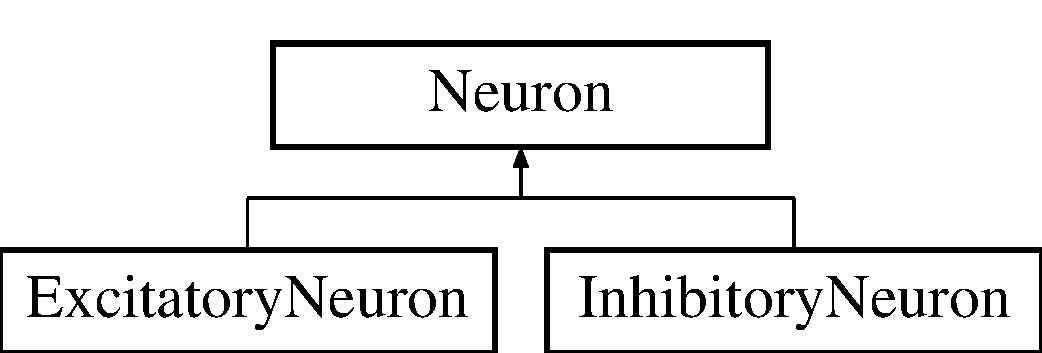
\includegraphics[height=2.000000cm]{classNeuron}
\end{center}
\end{figure}
\subsection*{Public Member Functions}
\begin{DoxyCompactItemize}
\item 
\hypertarget{classNeuron_a823487d01615fadb8ac19a2768dd9d96}{\hyperlink{classNeuron_a823487d01615fadb8ac19a2768dd9d96}{Neuron} ()}\label{classNeuron_a823487d01615fadb8ac19a2768dd9d96}

\begin{DoxyCompactList}\small\item\em A constructor. \end{DoxyCompactList}\item 
\hypertarget{classNeuron_a94a250ce7e167760e593979b899745b1}{virtual \hyperlink{classNeuron_a94a250ce7e167760e593979b899745b1}{$\sim$\-Neuron} ()}\label{classNeuron_a94a250ce7e167760e593979b899745b1}

\begin{DoxyCompactList}\small\item\em A destructor. \end{DoxyCompactList}\item 
double \hyperlink{classNeuron_a86341dee7a81765fe4840777a008c688}{get\-Membrane\-Potential} () const 
\begin{DoxyCompactList}\small\item\em A getter for the neuron's membrane potential. \end{DoxyCompactList}\item 
size\-\_\-t \hyperlink{classNeuron_a9497c01c1513b480cb96488e104c8b00}{get\-Number\-Of\-Spikes} () const 
\begin{DoxyCompactList}\small\item\em A getter for the number of times the neuron spiked in the course of time. \end{DoxyCompactList}\item 
void \hyperlink{classNeuron_ae77210c7b0bf3739b01ec2e3dba96827}{set\-Input\-Current} (double external\-Current)
\begin{DoxyCompactList}\small\item\em A setter for the external input current. \end{DoxyCompactList}\item 
void \hyperlink{classNeuron_a782b3b728eee5097ab205a7a7990225b}{update} ()
\begin{DoxyCompactList}\small\item\em Is invoked at each cycle of the simulation and makes the neutron evolve in the course of time. \end{DoxyCompactList}\item 
\hypertarget{classNeuron_ababbaa5bc5f7b2e00e0ae5ffcc8fbfdb}{void {\bfseries update\-Without\-Background\-Noise} ()}\label{classNeuron_ababbaa5bc5f7b2e00e0ae5ffcc8fbfdb}

\item 
\hypertarget{classNeuron_a521a967d65a078140cc9c6b8d30240ce}{void {\bfseries update} (void(Neuron\-::$\ast$membrane\-Potential\-Update)())}\label{classNeuron_a521a967d65a078140cc9c6b8d30240ce}

\item 
bool \hyperlink{classNeuron_aa40fbb2b025efb1db420da32e16741c1}{is\-Refractory} () const 
\item 
void \hyperlink{classNeuron_a955ecfd2984f75c18664bd370c34af1d}{spike} ()
\item 
void \hyperlink{classNeuron_aa8111a347de6ddfb6c799bdcd3092cb7}{receive\-Spike} (unsigned int local\-Time\-Of\-Spiking\-Neuron, double spike\-Amplitude)
\item 
void \hyperlink{classNeuron_a41a81d8527734e59bae39f73fece887f}{update\-Membrane\-Potential} ()
\item 
\hypertarget{classNeuron_a2a3d0130b76a6e1daa0191b97718178b}{void {\bfseries update\-Membrane\-Potential\-Without\-Background\-Noise} ()}\label{classNeuron_a2a3d0130b76a6e1daa0191b97718178b}

\item 
double \hyperlink{classNeuron_a763493ef8eff51a638cbb75f0983b828}{read\-Ring\-Buffer} () const 
\item 
void \hyperlink{classNeuron_a41dd9577d84a48bd427201b4b8234150}{reinitialize\-Current\-Ring\-Buffer\-Element} ()
\item 
size\-\_\-t \hyperlink{classNeuron_af1c7b80b5e70e906734ce710d37b1fd7}{time\-To\-Ring\-Buffer\-Index} (unsigned int time) const 
\item 
virtual double \hyperlink{classNeuron_aec2283fbfaba764cd088e6d16b0a74bb}{get\-Spike\-Amplitude} () const 
\item 
void \hyperlink{classNeuron_a15b3eaa67535301e011d5cd8d53a61d1}{print\-Spiking\-Times} (const std\-::string \&name\-Of\-File) const 
\item 
void \hyperlink{classNeuron_a9bf071c800e76fa7fbd611cee7cd76d6}{add\-Target} (\hyperlink{classNeuron}{Neuron} $\ast$target)
\item 
const std\-::vector$<$ unsigned int $>$ \& \hyperlink{classNeuron_ae87bb09d99e4e9c2185be8b73fc242ba}{get\-Spike\-Time} () const 
\item 
double \hyperlink{classNeuron_a5487631e8982ae2368da0917535a9001}{get\-Background\-Noise} () const 
\end{DoxyCompactItemize}


\subsection{Member Function Documentation}
\hypertarget{classNeuron_a9bf071c800e76fa7fbd611cee7cd76d6}{\index{Neuron@{Neuron}!add\-Target@{add\-Target}}
\index{add\-Target@{add\-Target}!Neuron@{Neuron}}
\subsubsection[{add\-Target}]{\setlength{\rightskip}{0pt plus 5cm}void Neuron\-::add\-Target (
\begin{DoxyParamCaption}
\item[{{\bf Neuron} $\ast$}]{target}
\end{DoxyParamCaption}
)}}\label{classNeuron_a9bf071c800e76fa7fbd611cee7cd76d6}
Establishes a connection to a postsynaptic neuron, by adding it to its target. 
\begin{DoxyParams}{Parameters}
{\em target,a} & pointer to a neuron that shall receive signals \\
\hline
\end{DoxyParams}
\hypertarget{classNeuron_a5487631e8982ae2368da0917535a9001}{\index{Neuron@{Neuron}!get\-Background\-Noise@{get\-Background\-Noise}}
\index{get\-Background\-Noise@{get\-Background\-Noise}!Neuron@{Neuron}}
\subsubsection[{get\-Background\-Noise}]{\setlength{\rightskip}{0pt plus 5cm}double Neuron\-::get\-Background\-Noise (
\begin{DoxyParamCaption}
{}
\end{DoxyParamCaption}
) const}}\label{classNeuron_a5487631e8982ae2368da0917535a9001}
Creates a value which accounts for the contribution of the rest of the brain. This contribution is modeled by Cext excitatory neurons that fire randomly according to a poisson distribution at a frequency vext. \begin{DoxySeeAlso}{See Also}
\hyperlink{classNeuron_a41a81d8527734e59bae39f73fece887f}{update\-Membrane\-Potential()} 
\end{DoxySeeAlso}
\begin{DoxyReturn}{Returns}
a randomly generated value representing the background noise coming from the rest of the brain, a double 
\end{DoxyReturn}
\hypertarget{classNeuron_a86341dee7a81765fe4840777a008c688}{\index{Neuron@{Neuron}!get\-Membrane\-Potential@{get\-Membrane\-Potential}}
\index{get\-Membrane\-Potential@{get\-Membrane\-Potential}!Neuron@{Neuron}}
\subsubsection[{get\-Membrane\-Potential}]{\setlength{\rightskip}{0pt plus 5cm}double Neuron\-::get\-Membrane\-Potential (
\begin{DoxyParamCaption}
{}
\end{DoxyParamCaption}
) const}}\label{classNeuron_a86341dee7a81765fe4840777a008c688}


A getter for the neuron's membrane potential. 

\begin{DoxyReturn}{Returns}
the neuron's membrane potential, a double 
\end{DoxyReturn}
\hypertarget{classNeuron_a9497c01c1513b480cb96488e104c8b00}{\index{Neuron@{Neuron}!get\-Number\-Of\-Spikes@{get\-Number\-Of\-Spikes}}
\index{get\-Number\-Of\-Spikes@{get\-Number\-Of\-Spikes}!Neuron@{Neuron}}
\subsubsection[{get\-Number\-Of\-Spikes}]{\setlength{\rightskip}{0pt plus 5cm}size\-\_\-t Neuron\-::get\-Number\-Of\-Spikes (
\begin{DoxyParamCaption}
{}
\end{DoxyParamCaption}
) const}}\label{classNeuron_a9497c01c1513b480cb96488e104c8b00}


A getter for the number of times the neuron spiked in the course of time. 

Uses the size of the vector storing the spike times. \begin{DoxyReturn}{Returns}
the number of times the neuon spiked, a size\-\_\-t 
\end{DoxyReturn}
\hypertarget{classNeuron_aec2283fbfaba764cd088e6d16b0a74bb}{\index{Neuron@{Neuron}!get\-Spike\-Amplitude@{get\-Spike\-Amplitude}}
\index{get\-Spike\-Amplitude@{get\-Spike\-Amplitude}!Neuron@{Neuron}}
\subsubsection[{get\-Spike\-Amplitude}]{\setlength{\rightskip}{0pt plus 5cm}double Neuron\-::get\-Spike\-Amplitude (
\begin{DoxyParamCaption}
{}
\end{DoxyParamCaption}
) const\hspace{0.3cm}{\ttfamily [virtual]}}}\label{classNeuron_aec2283fbfaba764cd088e6d16b0a74bb}
A virtual method which reads the constant spike amplitude, that differs between inhibitory and excitatory neurons, from the parameter file. (The method is defined for unspecified neurons as well so that the tests of previous versions of the program are still functional, otherwise it could be virtual pure.). \begin{DoxySeeAlso}{See Also}
\hyperlink{classNeuron_a41a81d8527734e59bae39f73fece887f}{update\-Membrane\-Potential()} 
\end{DoxySeeAlso}
\begin{DoxyReturn}{Returns}
the spike amplitudes of the presynaptic neuron, a double 
\end{DoxyReturn}


Reimplemented in \hyperlink{classExcitatoryNeuron_a7d38213943753c84022c52db84601e67}{Excitatory\-Neuron}, and \hyperlink{classInhibitoryNeuron_a762e2b7bcf64962f764031d991911b7a}{Inhibitory\-Neuron}.

\hypertarget{classNeuron_ae87bb09d99e4e9c2185be8b73fc242ba}{\index{Neuron@{Neuron}!get\-Spike\-Time@{get\-Spike\-Time}}
\index{get\-Spike\-Time@{get\-Spike\-Time}!Neuron@{Neuron}}
\subsubsection[{get\-Spike\-Time}]{\setlength{\rightskip}{0pt plus 5cm}const vector$<$ unsigned int $>$ \& Neuron\-::get\-Spike\-Time (
\begin{DoxyParamCaption}
{}
\end{DoxyParamCaption}
) const}}\label{classNeuron_ae87bb09d99e4e9c2185be8b73fc242ba}
A getter for the neuron's spike times. \begin{DoxyReturn}{Returns}
the neuron's spiking times in simulation steps, a vector of unsigned integers 
\end{DoxyReturn}
\hypertarget{classNeuron_aa40fbb2b025efb1db420da32e16741c1}{\index{Neuron@{Neuron}!is\-Refractory@{is\-Refractory}}
\index{is\-Refractory@{is\-Refractory}!Neuron@{Neuron}}
\subsubsection[{is\-Refractory}]{\setlength{\rightskip}{0pt plus 5cm}bool Neuron\-::is\-Refractory (
\begin{DoxyParamCaption}
{}
\end{DoxyParamCaption}
) const}}\label{classNeuron_aa40fbb2b025efb1db420da32e16741c1}
Compares the neuron's internal time to the time of the last spike and the refraction time in order to test if the neuron is in a refractory period. \begin{DoxySeeAlso}{See Also}
\hyperlink{classNeuron_a782b3b728eee5097ab205a7a7990225b}{update()} 
\end{DoxySeeAlso}
\begin{DoxyReturn}{Returns}
if the neuron is in a refractory state, a bool 
\end{DoxyReturn}
\hypertarget{classNeuron_a15b3eaa67535301e011d5cd8d53a61d1}{\index{Neuron@{Neuron}!print\-Spiking\-Times@{print\-Spiking\-Times}}
\index{print\-Spiking\-Times@{print\-Spiking\-Times}!Neuron@{Neuron}}
\subsubsection[{print\-Spiking\-Times}]{\setlength{\rightskip}{0pt plus 5cm}void Neuron\-::print\-Spiking\-Times (
\begin{DoxyParamCaption}
\item[{const std\-::string \&}]{name\-Of\-File}
\end{DoxyParamCaption}
) const}}\label{classNeuron_a15b3eaa67535301e011d5cd8d53a61d1}
Converts the times when the neuron spiked to milliseconds and stores these values in a file. 
\begin{DoxyParams}{Parameters}
{\em name\-Of\-File,a} & string \\
\hline
\end{DoxyParams}
\hypertarget{classNeuron_a763493ef8eff51a638cbb75f0983b828}{\index{Neuron@{Neuron}!read\-Ring\-Buffer@{read\-Ring\-Buffer}}
\index{read\-Ring\-Buffer@{read\-Ring\-Buffer}!Neuron@{Neuron}}
\subsubsection[{read\-Ring\-Buffer}]{\setlength{\rightskip}{0pt plus 5cm}double Neuron\-::read\-Ring\-Buffer (
\begin{DoxyParamCaption}
{}
\end{DoxyParamCaption}
) const}}\label{classNeuron_a763493ef8eff51a638cbb75f0983b828}
Reads the ring buffer's current entry to receive the spikes arriving with a delay that where emmited by presynaptic neurons. \begin{DoxySeeAlso}{See Also}
\hyperlink{classNeuron_a41a81d8527734e59bae39f73fece887f}{update\-Membrane\-Potential()} 
\end{DoxySeeAlso}
\begin{DoxyReturn}{Returns}
the sum of spike amplitudes of spikes from connected neurons that are currently arriving, a double 
\end{DoxyReturn}
\hypertarget{classNeuron_aa8111a347de6ddfb6c799bdcd3092cb7}{\index{Neuron@{Neuron}!receive\-Spike@{receive\-Spike}}
\index{receive\-Spike@{receive\-Spike}!Neuron@{Neuron}}
\subsubsection[{receive\-Spike}]{\setlength{\rightskip}{0pt plus 5cm}void Neuron\-::receive\-Spike (
\begin{DoxyParamCaption}
\item[{unsigned int}]{local\-Time\-Of\-Spiking\-Neuron, }
\item[{double}]{spike\-Amplitude}
\end{DoxyParamCaption}
)}}\label{classNeuron_aa8111a347de6ddfb6c799bdcd3092cb7}
This method of a connected neuron is called when the neuron spikes. The spike gets stored in its ring buffer in order to be read at the appropriate time. \begin{DoxySeeAlso}{See Also}
\hyperlink{classNeuron_a955ecfd2984f75c18664bd370c34af1d}{spike()} 
\end{DoxySeeAlso}

\begin{DoxyParams}{Parameters}
{\em local\-Time\-Of\-Spiking\-Neuron,an} & unsigned integer \\
\hline
{\em spike\-Amplitude,defining} & the strength of the signal \\
\hline
\end{DoxyParams}
\begin{DoxyReturn}{Returns}
if the neuron is in a refractory state, a bool 
\end{DoxyReturn}
\hypertarget{classNeuron_a41dd9577d84a48bd427201b4b8234150}{\index{Neuron@{Neuron}!reinitialize\-Current\-Ring\-Buffer\-Element@{reinitialize\-Current\-Ring\-Buffer\-Element}}
\index{reinitialize\-Current\-Ring\-Buffer\-Element@{reinitialize\-Current\-Ring\-Buffer\-Element}!Neuron@{Neuron}}
\subsubsection[{reinitialize\-Current\-Ring\-Buffer\-Element}]{\setlength{\rightskip}{0pt plus 5cm}void Neuron\-::reinitialize\-Current\-Ring\-Buffer\-Element (
\begin{DoxyParamCaption}
{}
\end{DoxyParamCaption}
)}}\label{classNeuron_a41dd9577d84a48bd427201b4b8234150}
Sets the current ring buffer element to zero and makes it thus ready to record new arriving spikes in another cycle to come. \begin{DoxySeeAlso}{See Also}
\hyperlink{classNeuron_a782b3b728eee5097ab205a7a7990225b}{update()} 
\end{DoxySeeAlso}
\hypertarget{classNeuron_ae77210c7b0bf3739b01ec2e3dba96827}{\index{Neuron@{Neuron}!set\-Input\-Current@{set\-Input\-Current}}
\index{set\-Input\-Current@{set\-Input\-Current}!Neuron@{Neuron}}
\subsubsection[{set\-Input\-Current}]{\setlength{\rightskip}{0pt plus 5cm}void Neuron\-::set\-Input\-Current (
\begin{DoxyParamCaption}
\item[{double}]{external\-Current}
\end{DoxyParamCaption}
)}}\label{classNeuron_ae77210c7b0bf3739b01ec2e3dba96827}


A setter for the external input current. 

A method allowing to simulate the stimulation of the neuron by an external current. Is invoked in the main loop of the simulation in order to indicate the strength of the external stimulus. 
\begin{DoxyParams}{Parameters}
{\em external\-Current,the} & external input current, a double. \\
\hline
\end{DoxyParams}
\hypertarget{classNeuron_a955ecfd2984f75c18664bd370c34af1d}{\index{Neuron@{Neuron}!spike@{spike}}
\index{spike@{spike}!Neuron@{Neuron}}
\subsubsection[{spike}]{\setlength{\rightskip}{0pt plus 5cm}void Neuron\-::spike (
\begin{DoxyParamCaption}
{}
\end{DoxyParamCaption}
)}}\label{classNeuron_a955ecfd2984f75c18664bd370c34af1d}
Stores the spiking time and sets the membrane potential to zero and sends an electrical impulse to the connected neurons. \begin{DoxySeeAlso}{See Also}
\hyperlink{classNeuron_a782b3b728eee5097ab205a7a7990225b}{update()} 
\end{DoxySeeAlso}
\hypertarget{classNeuron_af1c7b80b5e70e906734ce710d37b1fd7}{\index{Neuron@{Neuron}!time\-To\-Ring\-Buffer\-Index@{time\-To\-Ring\-Buffer\-Index}}
\index{time\-To\-Ring\-Buffer\-Index@{time\-To\-Ring\-Buffer\-Index}!Neuron@{Neuron}}
\subsubsection[{time\-To\-Ring\-Buffer\-Index}]{\setlength{\rightskip}{0pt plus 5cm}size\-\_\-t Neuron\-::time\-To\-Ring\-Buffer\-Index (
\begin{DoxyParamCaption}
\item[{unsigned int}]{time}
\end{DoxyParamCaption}
) const}}\label{classNeuron_af1c7b80b5e70e906734ce710d37b1fd7}
Auxilliary method that yields the associated ring buffer index to a a given time by means of the modulo operator and checks if it is licit. \begin{DoxySeeAlso}{See Also}
\hyperlink{classNeuron_aa8111a347de6ddfb6c799bdcd3092cb7}{receive\-Spike()} 

\hyperlink{classNeuron_a763493ef8eff51a638cbb75f0983b828}{read\-Ring\-Buffer()} 

\hyperlink{classNeuron_a41dd9577d84a48bd427201b4b8234150}{reinitialize\-Current\-Ring\-Buffer\-Element()} 
\end{DoxySeeAlso}

\begin{DoxyParams}{Parameters}
{\em the} & time of which one wants to know the corresponding ring buffer index, an unsigned integer \\
\hline
\end{DoxyParams}
\begin{DoxyReturn}{Returns}
the ring buffer index corresponding to the given time, a size\-\_\-t 
\end{DoxyReturn}
\hypertarget{classNeuron_a782b3b728eee5097ab205a7a7990225b}{\index{Neuron@{Neuron}!update@{update}}
\index{update@{update}!Neuron@{Neuron}}
\subsubsection[{update}]{\setlength{\rightskip}{0pt plus 5cm}void Neuron\-::update (
\begin{DoxyParamCaption}
{}
\end{DoxyParamCaption}
)}}\label{classNeuron_a782b3b728eee5097ab205a7a7990225b}


Is invoked at each cycle of the simulation and makes the neutron evolve in the course of time. 

Advances the neuron one step as a function of its current state by eventual spiking if the membrane potential has reached a threshold, resting inactive during the refractory period after a spike or updating the membrane potential and finally handling the ring buffer as well as incrementing the neuron's internal clock. \hypertarget{classNeuron_a41a81d8527734e59bae39f73fece887f}{\index{Neuron@{Neuron}!update\-Membrane\-Potential@{update\-Membrane\-Potential}}
\index{update\-Membrane\-Potential@{update\-Membrane\-Potential}!Neuron@{Neuron}}
\subsubsection[{update\-Membrane\-Potential}]{\setlength{\rightskip}{0pt plus 5cm}void Neuron\-::update\-Membrane\-Potential (
\begin{DoxyParamCaption}
{}
\end{DoxyParamCaption}
)}}\label{classNeuron_a41a81d8527734e59bae39f73fece887f}
Calculates and sets the new membrane potential as a function of the current membrane potential, the external input current, the spikes that arrived with a signal delay and the random background noise arriving from the rest of the brain. \begin{DoxySeeAlso}{See Also}
\hyperlink{classNeuron_a782b3b728eee5097ab205a7a7990225b}{update()} 
\end{DoxySeeAlso}


The documentation for this class was generated from the following files\-:\begin{DoxyCompactItemize}
\item 
/home/\-I\-N\-T\-R\-A\-N\-E\-T/bmarty/\-Desktop/myfiles/cpp/second\-Year/second\-Week/\-Neuron-\/\-Program/scr/neuron.\-hpp\item 
/home/\-I\-N\-T\-R\-A\-N\-E\-T/bmarty/\-Desktop/myfiles/cpp/second\-Year/second\-Week/\-Neuron-\/\-Program/scr/neuron.\-cpp\end{DoxyCompactItemize}

%--- End generated contents ---

% Index
\newpage
\phantomsection
\addcontentsline{toc}{chapter}{Index}
\printindex

\end{document}
